\section{Systembeskrivelse}
Der ønskes at udvikle et system, med formål at støtte musklerne omkring knæleddet hos ALS-patienter under udførelse af en squat-øvelse. Dette gøres for at aflaste patienterne med henblik på at kunne undgå kørestol i de tidlige stadier af ALS. 
Systemet skal kunne opsamle EMG-signaler fra rectus femoris samt en spænding fra de påsatte accelerometre, for således at kunne beregne vinklen over knæet. Disse signaler skal behandles således, at de kan omsættes til signaler, så en prototype af et exoskelet kan udføre en tilsvarende bevægelse. 
Systemet har yderligere til formål at have mulighed for forstærkning af signalet, således mindre muskelkraft også vil kunne udløse den samme bevægelse af knæleddet. 
Derudover skal systemet være brugervenligt ved at være kompakt, mobilt og ikke generende over for brugeren.

\subsection{Overordnet krav til systemet}  \label{sec:overordnet_krav}
\begin{itemize}
\item Systemet skal registrere muskelaktivitet af rectus femoris og vinklen af knæleddet
\item Systemet skal være batteridrevet
\item Systemet skal kunne overføre data trådløst til en computer
%\item Systemet skal kunne ende ud i en prototype af et exoskelet
\item Systemet skal være sikkert og ikke til gene for brugeren 
\item Systemet skal kunne indikere, hvis der ikke er strøm nok til at virke optimalt
\item Systemet skal reagere på kroppens naturlige bevægelse under en squat-øvelse, så det vil kunne benyttes til en prototype af et exoskelet
\end{itemize}


\subsection{Blokdiagram} \label{sec:blokdiagram} 
\begin{figure}[H]
\centering
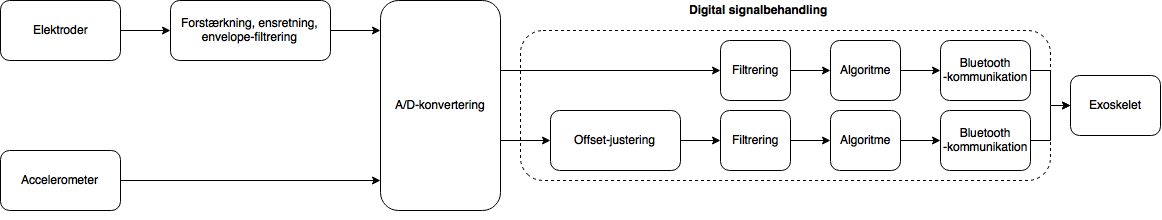
\includegraphics[width=1\textwidth]{figures/blokdiagram.png}
\caption{Systemets opbygning.}
\label{fig:blokdiagram}
\end{figure}

\noindent
I dette projekt er der valgt at udarbejde en prototype, som har til formål at bevæge knæleddet, når rectus femoris kontraherer. Opbygningen af systemet fremgår af \autoref{fig:blokdiagram}. Der anvendes to sensorer, EMG-elekroder og accelerometre, til at opsamle biologiske signaler. 
For at registrere muskelaktivitet anvendes elektroder og en EMG-forstærker, der har til formål at forstærke, filtrere og ensrette muskelsignalet, der opsamles. 
Der anvendes accelerometre som inputsignal. Inputsignalet omregnes til en vinkel svarende til knæleddets vinkel under en squat-øvelse. 
De opsamlede signaler sendes herefter videre til den digitale del af systemet, hvilket er bestående af et Bluetooth Low Energy Pioneer kit (CY8CKIT-042-BLE), som opfanger de biologiske signaler og overfører dem trådløst til en CySmartUSB BLE Dongle sat i en computer, som kan kommunikere med prototypen af exoskelettet udarbejdet i LEGO Mindstorm \fxnote{tjek om dette er rigtigt}. 

